% Example talk for the uoc theme.
%
% Format: wide (16:9) by default. For the standard format (4:3), change 169 to 43 below,
% or build with `just build example 43`, which defines \aspect before this line.
\providecommand{\aspect}{169}
\documentclass[aspectratio=\aspect, 10pt]{beamer}
\usetheme{uoc}
% Notes version: compile example-notes.tex (slides on the left, notes on the right)
\ifdefined\shownotes
  \usepackage{pgfpages}
  \setbeameroption{show notes on second screen=right}
\fi
\graphicspath{{../tikz/}}

% Bold vectors and matrices (kpfonts-otf loads unicode-math)
\usepackage{mathtools}
\newcommand{\bm}[1]{\symbfit{#1}}
\newcommand{\Real}{\mathbb{R}}

% Code listings in the slide colors
\usepackage{listings}
\lstset{
  language=Python,
  basicstyle=\ttfamily\small,
  keywordstyle=\color{teal}\bfseries,
  commentstyle=\color{softgray},
  columns=fullflexible,
  keepspaces=true,
  showstringspaces=false,
}

\title{Learning operators with neural networks}
\subtitle{Example talk for the presentation template}
\author{Georgios Arampatzis}
\institute{Department of Mathematics \& Applied Mathematics, University of Crete\\
  Institute of Applied \& Computational Mathematics, FORTH}
\date{\today}

\begin{document}

\maketitle

\begin{frame}{Outline}
  \begin{itemize}
    \item Gradients by reverse-mode automatic differentiation
    \item Recurrent networks for time series
    \item Neural operators: DeepONet and the Fourier neural operator
  \end{itemize}
\end{frame}
\note[itemize]{
  \item One sentence per part: what it is for.
  \item \nextslide reverse mode on a small example.
}

\section{Automatic differentiation}

\begin{frame}[c]{Reverse mode on a computational graph}
  \centering
  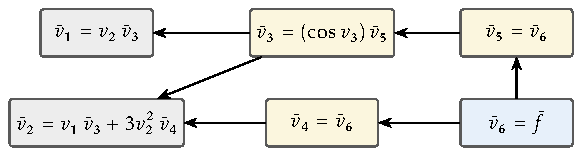
\includegraphics[max width=\textwidth]{ad_graph_reverse}
  \source{Graph of $f(x_1,x_2)=\sin(x_1x_2)+x_2^3$. Each node holds its adjoint $\bar v_i=\partial f/\partial v_i$.}
\end{frame}
\note{One reverse sweep gives the derivatives with respect to both inputs.}

\begin{frame}{Cost of reverse mode}
  \begin{itemize}
    \item A \term{reverse sweep} visits each node once, from the output back to the inputs.
    \item The full gradient costs a small constant times one evaluation of $f$.
      \calc{For $f:\Real^n\to\Real$, forward mode needs $n$ sweeps and reverse mode needs one.}
    \item \alert{The price is memory}: every intermediate value is stored for the reverse sweep.
  \end{itemize}
  \begin{block}{Theorem (cost of the gradient)}
    For $f:\Real^n\to\Real$ evaluated in time $T$, reverse mode returns $\nabla f$ in time at most $cT$,
    with a constant $c$ independent of $n$.
  \end{block}
\end{frame}

\section{Recurrent networks}

\begin{frame}[c]{One LSTM cell}
  \centering
  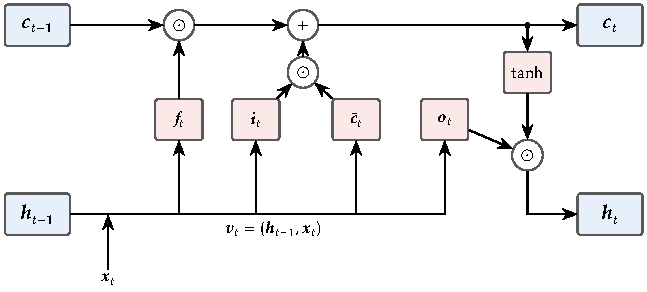
\includegraphics[max width=\textwidth]{lstm_cell}
  \source{The cell state $\bm c_t$ runs across the top; the gates $\bm f_t$, $\bm i_t$, and $\bm o_t$ act by elementwise products.}
\end{frame}

\begin{frame}[fragile]{The LSTM cell in code}
\begin{lstlisting}
def lstm_cell(h, c, x, W, b):
    v = concat(h, x)
    f, i, g, o = split(W @ v + b, 4)
    c = sigmoid(f) * c + sigmoid(i) * tanh(g)
    h = sigmoid(o) * tanh(c)
    return h, c
\end{lstlisting}
  \begin{itemize}
    \item One matrix product gives all four gates.
    \item The update of $\bm c_t$ is additive, so its gradient passes through many steps.
  \end{itemize}
\end{frame}

\section{Neural operators}

\begin{frame}[c]{DeepONet}
  \centering
  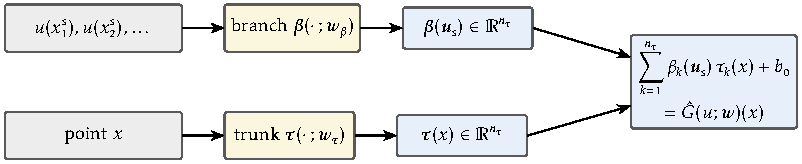
\includegraphics[max width=\textwidth]{deeponet_net}
  \source{The branch network reads the input function $u$ at the sensors; the trunk network reads the point $x$.}
\end{frame}

\begin{frame}[c]{Fourier neural operator}
  \centering
  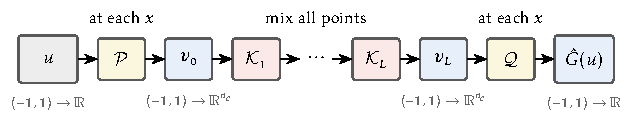
\includegraphics[max width=\textwidth]{fno_net}
  \source{A pointwise lifting $\mathcal P$, $L$ Fourier layers, and a pointwise projection $\mathcal Q$.}
\end{frame}

\begin{frame}{Comparison}
  \centering
  \begin{tabular}{lcc}
    \toprule
    & DeepONet & FNO \\
    \midrule
    Input function    & values at fixed sensors & values on a grid \\
    Output            & any point $x$           & the same grid \\
    \hlrow Main cost  & two networks            & FFT per layer \\
    \bottomrule
  \end{tabular}
  \source{Highlighted row: the operation that sets the training time.}
\end{frame}

\begin{frame}[standout]
  Thank you\\[2ex]
  {\normalsize\mdseries georgios.arampatzis@uoc.gr}
\end{frame}

\end{document}
